% Options for packages loaded elsewhere
\PassOptionsToPackage{unicode}{hyperref}
\PassOptionsToPackage{hyphens}{url}
%
\documentclass[
]{article}
\usepackage{amsmath,amssymb}
\usepackage{iftex}
\ifPDFTeX
  \usepackage[T1]{fontenc}
  \usepackage[utf8]{inputenc}
  \usepackage{textcomp} % provide euro and other symbols
\else % if luatex or xetex
  \usepackage{unicode-math} % this also loads fontspec
  \defaultfontfeatures{Scale=MatchLowercase}
  \defaultfontfeatures[\rmfamily]{Ligatures=TeX,Scale=1}
\fi
\usepackage{lmodern}
\ifPDFTeX\else
  % xetex/luatex font selection
\fi
% Use upquote if available, for straight quotes in verbatim environments
\IfFileExists{upquote.sty}{\usepackage{upquote}}{}
\IfFileExists{microtype.sty}{% use microtype if available
  \usepackage[]{microtype}
  \UseMicrotypeSet[protrusion]{basicmath} % disable protrusion for tt fonts
}{}
\makeatletter
\@ifundefined{KOMAClassName}{% if non-KOMA class
  \IfFileExists{parskip.sty}{%
    \usepackage{parskip}
  }{% else
    \setlength{\parindent}{0pt}
    \setlength{\parskip}{6pt plus 2pt minus 1pt}}
}{% if KOMA class
  \KOMAoptions{parskip=half}}
\makeatother
\usepackage{xcolor}
\usepackage[margin=1in]{geometry}
\usepackage{color}
\usepackage{fancyvrb}
\newcommand{\VerbBar}{|}
\newcommand{\VERB}{\Verb[commandchars=\\\{\}]}
\DefineVerbatimEnvironment{Highlighting}{Verbatim}{commandchars=\\\{\}}
% Add ',fontsize=\small' for more characters per line
\usepackage{framed}
\definecolor{shadecolor}{RGB}{248,248,248}
\newenvironment{Shaded}{\begin{snugshade}}{\end{snugshade}}
\newcommand{\AlertTok}[1]{\textcolor[rgb]{0.94,0.16,0.16}{#1}}
\newcommand{\AnnotationTok}[1]{\textcolor[rgb]{0.56,0.35,0.01}{\textbf{\textit{#1}}}}
\newcommand{\AttributeTok}[1]{\textcolor[rgb]{0.13,0.29,0.53}{#1}}
\newcommand{\BaseNTok}[1]{\textcolor[rgb]{0.00,0.00,0.81}{#1}}
\newcommand{\BuiltInTok}[1]{#1}
\newcommand{\CharTok}[1]{\textcolor[rgb]{0.31,0.60,0.02}{#1}}
\newcommand{\CommentTok}[1]{\textcolor[rgb]{0.56,0.35,0.01}{\textit{#1}}}
\newcommand{\CommentVarTok}[1]{\textcolor[rgb]{0.56,0.35,0.01}{\textbf{\textit{#1}}}}
\newcommand{\ConstantTok}[1]{\textcolor[rgb]{0.56,0.35,0.01}{#1}}
\newcommand{\ControlFlowTok}[1]{\textcolor[rgb]{0.13,0.29,0.53}{\textbf{#1}}}
\newcommand{\DataTypeTok}[1]{\textcolor[rgb]{0.13,0.29,0.53}{#1}}
\newcommand{\DecValTok}[1]{\textcolor[rgb]{0.00,0.00,0.81}{#1}}
\newcommand{\DocumentationTok}[1]{\textcolor[rgb]{0.56,0.35,0.01}{\textbf{\textit{#1}}}}
\newcommand{\ErrorTok}[1]{\textcolor[rgb]{0.64,0.00,0.00}{\textbf{#1}}}
\newcommand{\ExtensionTok}[1]{#1}
\newcommand{\FloatTok}[1]{\textcolor[rgb]{0.00,0.00,0.81}{#1}}
\newcommand{\FunctionTok}[1]{\textcolor[rgb]{0.13,0.29,0.53}{\textbf{#1}}}
\newcommand{\ImportTok}[1]{#1}
\newcommand{\InformationTok}[1]{\textcolor[rgb]{0.56,0.35,0.01}{\textbf{\textit{#1}}}}
\newcommand{\KeywordTok}[1]{\textcolor[rgb]{0.13,0.29,0.53}{\textbf{#1}}}
\newcommand{\NormalTok}[1]{#1}
\newcommand{\OperatorTok}[1]{\textcolor[rgb]{0.81,0.36,0.00}{\textbf{#1}}}
\newcommand{\OtherTok}[1]{\textcolor[rgb]{0.56,0.35,0.01}{#1}}
\newcommand{\PreprocessorTok}[1]{\textcolor[rgb]{0.56,0.35,0.01}{\textit{#1}}}
\newcommand{\RegionMarkerTok}[1]{#1}
\newcommand{\SpecialCharTok}[1]{\textcolor[rgb]{0.81,0.36,0.00}{\textbf{#1}}}
\newcommand{\SpecialStringTok}[1]{\textcolor[rgb]{0.31,0.60,0.02}{#1}}
\newcommand{\StringTok}[1]{\textcolor[rgb]{0.31,0.60,0.02}{#1}}
\newcommand{\VariableTok}[1]{\textcolor[rgb]{0.00,0.00,0.00}{#1}}
\newcommand{\VerbatimStringTok}[1]{\textcolor[rgb]{0.31,0.60,0.02}{#1}}
\newcommand{\WarningTok}[1]{\textcolor[rgb]{0.56,0.35,0.01}{\textbf{\textit{#1}}}}
\usepackage{graphicx}
\makeatletter
\def\maxwidth{\ifdim\Gin@nat@width>\linewidth\linewidth\else\Gin@nat@width\fi}
\def\maxheight{\ifdim\Gin@nat@height>\textheight\textheight\else\Gin@nat@height\fi}
\makeatother
% Scale images if necessary, so that they will not overflow the page
% margins by default, and it is still possible to overwrite the defaults
% using explicit options in \includegraphics[width, height, ...]{}
\setkeys{Gin}{width=\maxwidth,height=\maxheight,keepaspectratio}
% Set default figure placement to htbp
\makeatletter
\def\fps@figure{htbp}
\makeatother
\setlength{\emergencystretch}{3em} % prevent overfull lines
\providecommand{\tightlist}{%
  \setlength{\itemsep}{0pt}\setlength{\parskip}{0pt}}
\setcounter{secnumdepth}{-\maxdimen} % remove section numbering
\ifLuaTeX
  \usepackage{selnolig}  % disable illegal ligatures
\fi
\usepackage{bookmark}
\IfFileExists{xurl.sty}{\usepackage{xurl}}{} % add URL line breaks if available
\urlstyle{same}
\hypersetup{
  pdftitle={Functional Trait Data!},
  pdfauthor={Kauanoe Greene},
  hidelinks,
  pdfcreator={LaTeX via pandoc}}

\title{Functional Trait Data!}
\author{Kauanoe Greene}
\date{2024-10-24}

\begin{document}
\maketitle

{
\setcounter{tocdepth}{2}
\tableofcontents
}
\begin{Shaded}
\begin{Highlighting}[]
\CommentTok{\# LIBRARIES}

\CommentTok{\# visuals}
\FunctionTok{library}\NormalTok{(tidyverse)}
\FunctionTok{library}\NormalTok{(tidytext)}
\FunctionTok{library}\NormalTok{(here)}

\CommentTok{\# models (stats)}
\FunctionTok{library}\NormalTok{(lmerTest)}
\FunctionTok{library}\NormalTok{ (RLRsim)}
\FunctionTok{library}\NormalTok{(Matrix)}
\CommentTok{\# library(lme4)}
\FunctionTok{library}\NormalTok{(lattice)}
\FunctionTok{library}\NormalTok{(car)}
\FunctionTok{library}\NormalTok{(nlme)}

\CommentTok{\# PACKAGES}
\CommentTok{\# install.packages(LaTeX)}
\end{Highlighting}
\end{Shaded}

\begin{Shaded}
\begin{Highlighting}[]
\NormalTok{cleandata }\OtherTok{\textless{}{-}} \FunctionTok{read\_csv}\NormalTok{(}\FunctionTok{here}\NormalTok{(}\StringTok{"Project"}\NormalTok{, }\StringTok{"Data"}\NormalTok{, }\StringTok{"cleandata.csv"}\NormalTok{))}
\FunctionTok{view}\NormalTok{(cleandata)}
\end{Highlighting}
\end{Shaded}

\section{Data Upload and Clean}\label{data-upload-and-clean}

\begin{Shaded}
\begin{Highlighting}[]
\CommentTok{\# DATA ANALYSES: Means}

\NormalTok{means }\OtherTok{\textless{}{-}}\NormalTok{ cleandata }\SpecialCharTok{\%\textgreater{}\%} 
  \FunctionTok{group\_by}\NormalTok{(Population, Week, Treatment) }\SpecialCharTok{\%\textgreater{}\%} 
  \FunctionTok{summarise}\NormalTok{(}\AttributeTok{mean.cond =} \FunctionTok{mean}\NormalTok{(Conductance, }\AttributeTok{na.rm =} \ConstantTok{TRUE}\NormalTok{), }
            \AttributeTok{mean.chl =} \FunctionTok{mean}\NormalTok{(Chlorophyll, }\AttributeTok{na.rm =} \ConstantTok{TRUE}\NormalTok{), }
            \AttributeTok{mean.alpha =} \FunctionTok{mean}\NormalTok{(Alpha, }\AttributeTok{na.rm =} \ConstantTok{TRUE}\NormalTok{), }
            \AttributeTok{mean.etrm=} \FunctionTok{mean}\NormalTok{(ETRmax, }\AttributeTok{na.rm =} \ConstantTok{TRUE}\NormalTok{), }
            \AttributeTok{mean.ek =} \FunctionTok{mean}\NormalTok{(Ek, }\AttributeTok{na.rm =} \ConstantTok{TRUE}\NormalTok{), }
            \AttributeTok{mean.npq =} \FunctionTok{mean}\NormalTok{(NPQmax, }\AttributeTok{na.rm =} \ConstantTok{TRUE}\NormalTok{), }
            \AttributeTok{mean.fvfm =} \FunctionTok{mean}\NormalTok{(FvFm, }\AttributeTok{na.rm =} \ConstantTok{TRUE}\NormalTok{))}
\end{Highlighting}
\end{Shaded}

\section{Data Visualization}\label{data-visualization}

\begin{Shaded}
\begin{Highlighting}[]
\CommentTok{\# CONDUCTANCE PLOT}
\CommentTok{\# Let us create a plot that will communicate our key takeaway}
\CommentTok{\# Main question: how does drought affect the performance of plants across populations, measured via stomatal conductance?}
\CommentTok{\# Key finding: stomatal conductance varies amongst control and drought treatment groups across populations over time.}
\CommentTok{\# Stomatal conductance data was collected on a weekly basis}

\NormalTok{conductanceplot }\OtherTok{\textless{}{-}}\NormalTok{ means }\SpecialCharTok{\%\textgreater{}\%} \CommentTok{\# datasheet}
  \FunctionTok{ggplot}\NormalTok{(}\FunctionTok{aes}\NormalTok{(}\AttributeTok{x =}\NormalTok{ Week, }\CommentTok{\# x{-}axis}
             \AttributeTok{y =}\NormalTok{ mean.cond, }\CommentTok{\# y{-}axis}
             \AttributeTok{color =}\NormalTok{ Treatment)) }\SpecialCharTok{+} \CommentTok{\# colors}
  \FunctionTok{geom\_point}\NormalTok{() }\SpecialCharTok{+}  \CommentTok{\# data points}
  \FunctionTok{geom\_line}\NormalTok{() }\SpecialCharTok{+}  \CommentTok{\# plot}
  \FunctionTok{labs}\NormalTok{(}\AttributeTok{subtitle =} \StringTok{"Detecting intraspecific variation in plasticity of rates of stomatal conductance in response to drought stress"}\NormalTok{, }\CommentTok{\# plot subtitle}
       \AttributeTok{caption =} \StringTok{"Data sourced from: Greene 2023"}\NormalTok{, }\CommentTok{\# plot caption}
       \AttributeTok{x =} \StringTok{"Time (Weeks)"}\NormalTok{, }\CommentTok{\# x{-}axis label}
       \AttributeTok{y =} \StringTok{"Mean Stomatal Conductance (mmol m\^{}({-}2) s\^{}({-}1)"}\NormalTok{) }\SpecialCharTok{+} \CommentTok{\# y{-}axis label}
  \FunctionTok{ggtitle}\NormalTok{(}\StringTok{"Effects of Drought on Leaf Stomatal Conductance in \textquotesingle{}A\textquotesingle{}ali\textquotesingle{}i"}\NormalTok{) }\SpecialCharTok{+} \CommentTok{\# plot title}
  \FunctionTok{facet\_wrap}\NormalTok{(}\SpecialCharTok{\textasciitilde{}}\NormalTok{Population) }\SpecialCharTok{+} \CommentTok{\# create panels for each population!}
  \FunctionTok{scale\_color\_manual}\NormalTok{(}\AttributeTok{breaks=} \FunctionTok{c}\NormalTok{(}\StringTok{"C"}\NormalTok{, }\StringTok{"PD"}\NormalTok{), }\AttributeTok{labels =} \FunctionTok{c}\NormalTok{(}\StringTok{"Control Group"}\NormalTok{, }\StringTok{"Pulse Drought Group"}\NormalTok{), }\AttributeTok{values =} \FunctionTok{c}\NormalTok{(}\StringTok{"darkblue"}\NormalTok{, }\StringTok{"maroon"}\NormalTok{)) }\SpecialCharTok{+} \CommentTok{\# rename legend variables}
  \FunctionTok{theme}\NormalTok{(}\AttributeTok{plot.title =} \FunctionTok{element\_text}\NormalTok{(}\AttributeTok{face =} \StringTok{"bold"}\NormalTok{, }\AttributeTok{color =} \StringTok{"black"}\NormalTok{, }\AttributeTok{hjust =} \FloatTok{0.5}\NormalTok{), }\CommentTok{\# bold title}
        \AttributeTok{axis.text.x =} \FunctionTok{element\_text}\NormalTok{(}\AttributeTok{size =} \DecValTok{8}\NormalTok{), }\AttributeTok{axis.title.x =} \FunctionTok{element\_text}\NormalTok{(}\AttributeTok{size =} \DecValTok{10}\NormalTok{), }\CommentTok{\# adjust x{-}axis labels}
        \AttributeTok{axis.text.y =} \FunctionTok{element\_text}\NormalTok{(}\AttributeTok{size =} \DecValTok{8}\NormalTok{), }\AttributeTok{axis.title.y =} \FunctionTok{element\_text}\NormalTok{(}\AttributeTok{size =} \DecValTok{10}\NormalTok{),   }\CommentTok{\# adjust y{-}axis labels}
        \AttributeTok{legend.position =} \StringTok{"top"}\NormalTok{, }
        \AttributeTok{plot.subtitle =} \FunctionTok{element\_text}\NormalTok{(}\AttributeTok{size =} \DecValTok{10}\NormalTok{, }\AttributeTok{hjust =} \FloatTok{0.5}\NormalTok{), }
        \AttributeTok{legend.title =} \FunctionTok{element\_blank}\NormalTok{())}

\CommentTok{\# save plot to my output folder}
\FunctionTok{ggsave}\NormalTok{(}\FunctionTok{here}\NormalTok{(}\StringTok{"Project"}\NormalTok{, }\StringTok{"Output"}\NormalTok{, }\StringTok{"conductanceplot.png"}\NormalTok{)) }

\CommentTok{\# view plot}
\NormalTok{conductanceplot}
\end{Highlighting}
\end{Shaded}

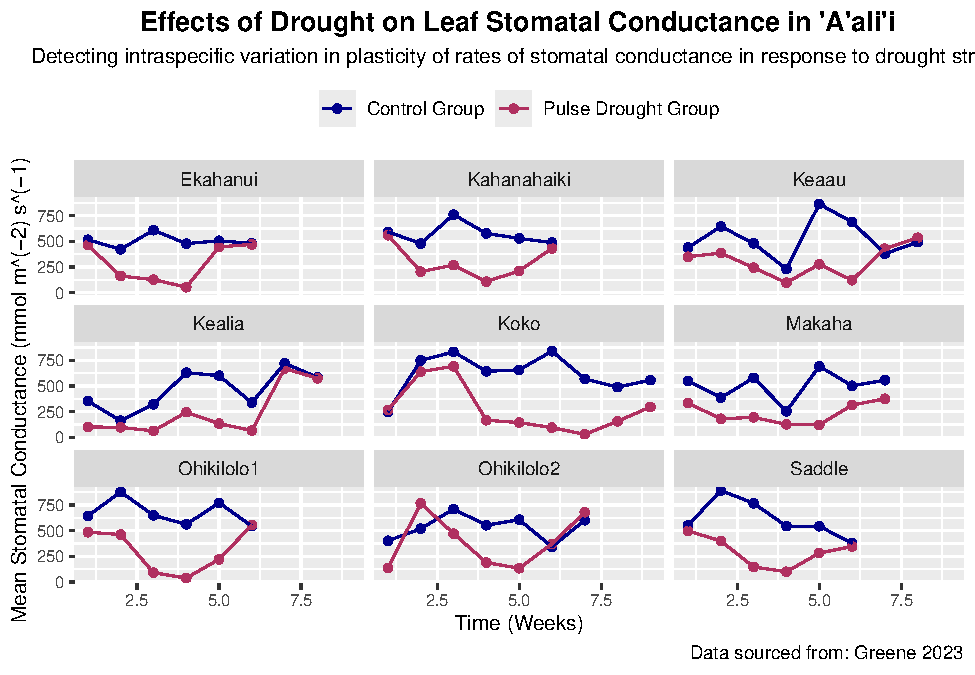
\includegraphics{../Output/unnamed-chunk-1-1.pdf}

\begin{Shaded}
\begin{Highlighting}[]
\NormalTok{chlplot }\OtherTok{\textless{}{-}}\NormalTok{ means }\SpecialCharTok{\%\textgreater{}\%} \CommentTok{\# datasheet}
  \FunctionTok{ggplot}\NormalTok{(}\FunctionTok{aes}\NormalTok{(}\AttributeTok{x =}\NormalTok{ Week, }\CommentTok{\# x{-}axis}
             \AttributeTok{y =}\NormalTok{ mean.chl, }\CommentTok{\# y{-}axis}
             \AttributeTok{color =}\NormalTok{ Treatment)) }\SpecialCharTok{+} \CommentTok{\# colors}
  \FunctionTok{geom\_point}\NormalTok{() }\SpecialCharTok{+}  \CommentTok{\# data points}
  \FunctionTok{geom\_line}\NormalTok{() }\SpecialCharTok{+}  \CommentTok{\# plot}
  \FunctionTok{labs}\NormalTok{(}\AttributeTok{subtitle =} \StringTok{"Detecting intraspecific variation in plasticity of rates of chlorophyll content in response to drought stress"}\NormalTok{, }\CommentTok{\# plot subtitle}
       \AttributeTok{caption =} \StringTok{"Data sourced from: Greene 2023"}\NormalTok{, }\CommentTok{\# plot caption}
       \AttributeTok{x =} \StringTok{"Time (Weeks)"}\NormalTok{, }\CommentTok{\# x{-}axis label}
       \AttributeTok{y =} \StringTok{"Mean Chlorophyll Content"}\NormalTok{) }\SpecialCharTok{+} \CommentTok{\# y{-}axis label}
  \FunctionTok{ggtitle}\NormalTok{(}\StringTok{"Effects of Drought on Leaf Chlorophyll Content in \textquotesingle{}A\textquotesingle{}ali\textquotesingle{}i"}\NormalTok{) }\SpecialCharTok{+} \CommentTok{\# plot title}
  \FunctionTok{facet\_wrap}\NormalTok{(}\SpecialCharTok{\textasciitilde{}}\NormalTok{Population) }\SpecialCharTok{+} \CommentTok{\# create panels for each population!}
  \FunctionTok{scale\_color\_manual}\NormalTok{(}\AttributeTok{breaks=} \FunctionTok{c}\NormalTok{(}\StringTok{"C"}\NormalTok{, }\StringTok{"PD"}\NormalTok{), }\AttributeTok{labels =} \FunctionTok{c}\NormalTok{(}\StringTok{"Control Group"}\NormalTok{, }\StringTok{"Pulse Drought Group"}\NormalTok{), }\AttributeTok{values =} \FunctionTok{c}\NormalTok{(}\StringTok{"darkgreen"}\NormalTok{, }\StringTok{"brown"}\NormalTok{)) }\SpecialCharTok{+} \CommentTok{\# rename legend variables}
  \FunctionTok{theme}\NormalTok{(}\AttributeTok{plot.title =} \FunctionTok{element\_text}\NormalTok{(}\AttributeTok{face =} \StringTok{"bold"}\NormalTok{, }\AttributeTok{color =} \StringTok{"black"}\NormalTok{, }\AttributeTok{hjust =} \FloatTok{0.5}\NormalTok{), }\CommentTok{\# bold title}
        \AttributeTok{axis.text.x =} \FunctionTok{element\_text}\NormalTok{(}\AttributeTok{size =} \DecValTok{8}\NormalTok{), }\AttributeTok{axis.title.x =} \FunctionTok{element\_text}\NormalTok{(}\AttributeTok{size =} \DecValTok{10}\NormalTok{), }\CommentTok{\# adjust x{-}axis labels}
        \AttributeTok{axis.text.y =} \FunctionTok{element\_text}\NormalTok{(}\AttributeTok{size =} \DecValTok{8}\NormalTok{), }\AttributeTok{axis.title.y =} \FunctionTok{element\_text}\NormalTok{(}\AttributeTok{size =} \DecValTok{10}\NormalTok{),   }\CommentTok{\# adjust y{-}axis labels}
        \AttributeTok{legend.position =} \StringTok{"top"}\NormalTok{, }
        \AttributeTok{plot.subtitle =} \FunctionTok{element\_text}\NormalTok{(}\AttributeTok{size =} \DecValTok{10}\NormalTok{, }\AttributeTok{hjust =} \FloatTok{0.5}\NormalTok{), }
        \AttributeTok{legend.title =} \FunctionTok{element\_blank}\NormalTok{())}

\CommentTok{\# save plot to my output folder}
\FunctionTok{ggsave}\NormalTok{(}\FunctionTok{here}\NormalTok{(}\StringTok{"Project"}\NormalTok{, }\StringTok{"Output"}\NormalTok{, }\StringTok{"chlplot.png"}\NormalTok{)) }

\CommentTok{\# view plot}
\NormalTok{chlplot}
\end{Highlighting}
\end{Shaded}

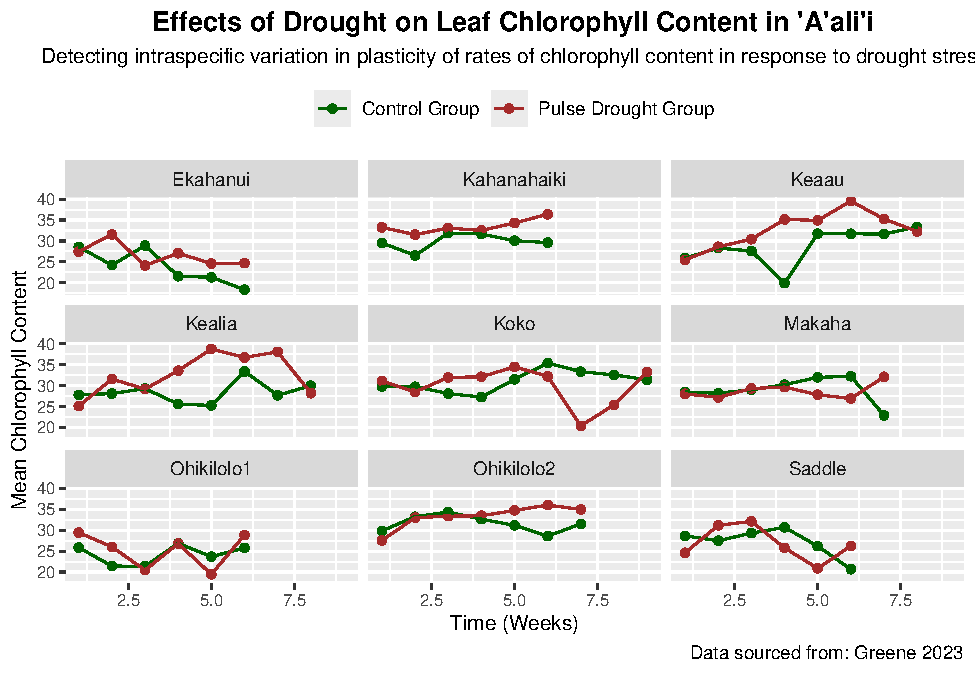
\includegraphics{../Output/unnamed-chunk-2-1.pdf}

\begin{Shaded}
\begin{Highlighting}[]
\NormalTok{fvfmplot }\OtherTok{\textless{}{-}}\NormalTok{ means }\SpecialCharTok{\%\textgreater{}\%} \CommentTok{\# datasheet}
  \FunctionTok{ggplot}\NormalTok{(}\FunctionTok{aes}\NormalTok{(}\AttributeTok{x =}\NormalTok{ Week, }\CommentTok{\# x{-}axis}
             \AttributeTok{y =}\NormalTok{ mean.fvfm, }\CommentTok{\# y{-}axis}
             \AttributeTok{color =}\NormalTok{ Treatment)) }\SpecialCharTok{+} \CommentTok{\# colors}
  \FunctionTok{geom\_point}\NormalTok{() }\SpecialCharTok{+}  \CommentTok{\# data points}
  \FunctionTok{geom\_line}\NormalTok{() }\SpecialCharTok{+}  \CommentTok{\# plot}
  \FunctionTok{labs}\NormalTok{(}\AttributeTok{subtitle =} \StringTok{"Detecting intraspecific variation in plasticity of photsynthetic yield in response to drought stress"}\NormalTok{, }\CommentTok{\# plot subtitle}
       \AttributeTok{caption =} \StringTok{"Data sourced from: Greene 2023"}\NormalTok{, }\CommentTok{\# plot caption}
       \AttributeTok{x =} \StringTok{"Time (Weeks)"}\NormalTok{, }\CommentTok{\# x{-}axis label}
       \AttributeTok{y =} \StringTok{"Mean Fv/Fm"}\NormalTok{) }\SpecialCharTok{+} \CommentTok{\# y{-}axis label}
  \FunctionTok{ggtitle}\NormalTok{(}\StringTok{"Effects of Drought on Leaf Stomatal Conductance in \textquotesingle{}A\textquotesingle{}ali\textquotesingle{}i"}\NormalTok{) }\SpecialCharTok{+} \CommentTok{\# plot title}
  \FunctionTok{facet\_wrap}\NormalTok{(}\SpecialCharTok{\textasciitilde{}}\NormalTok{Population) }\SpecialCharTok{+} \CommentTok{\# create panels for each population!}
  \FunctionTok{scale\_color\_manual}\NormalTok{(}\AttributeTok{breaks=} \FunctionTok{c}\NormalTok{(}\StringTok{"C"}\NormalTok{, }\StringTok{"PD"}\NormalTok{), }\AttributeTok{labels =} \FunctionTok{c}\NormalTok{(}\StringTok{"Control Group"}\NormalTok{, }\StringTok{"Pulse Drought Group"}\NormalTok{), }\AttributeTok{values =} \FunctionTok{c}\NormalTok{(}\StringTok{"orange"}\NormalTok{, }\StringTok{"maroon"}\NormalTok{)) }\SpecialCharTok{+} \CommentTok{\# rename legend variables}
  \FunctionTok{theme}\NormalTok{(}\AttributeTok{plot.title =} \FunctionTok{element\_text}\NormalTok{(}\AttributeTok{face =} \StringTok{"bold"}\NormalTok{, }\AttributeTok{color =} \StringTok{"black"}\NormalTok{, }\AttributeTok{hjust =} \FloatTok{0.5}\NormalTok{), }\CommentTok{\# bold title}
        \AttributeTok{axis.text.x =} \FunctionTok{element\_text}\NormalTok{(}\AttributeTok{size =} \DecValTok{8}\NormalTok{), }\AttributeTok{axis.title.x =} \FunctionTok{element\_text}\NormalTok{(}\AttributeTok{size =} \DecValTok{10}\NormalTok{), }\CommentTok{\# adjust x{-}axis labels}
        \AttributeTok{axis.text.y =} \FunctionTok{element\_text}\NormalTok{(}\AttributeTok{size =} \DecValTok{8}\NormalTok{), }\AttributeTok{axis.title.y =} \FunctionTok{element\_text}\NormalTok{(}\AttributeTok{size =} \DecValTok{10}\NormalTok{),   }\CommentTok{\# adjust y{-}axis labels}
        \AttributeTok{legend.position =} \StringTok{"top"}\NormalTok{, }
        \AttributeTok{plot.subtitle =} \FunctionTok{element\_text}\NormalTok{(}\AttributeTok{size =} \DecValTok{10}\NormalTok{, }\AttributeTok{hjust =} \FloatTok{0.5}\NormalTok{), }
        \AttributeTok{legend.title =} \FunctionTok{element\_blank}\NormalTok{())}

\CommentTok{\# save plot to my output folder}
\FunctionTok{ggsave}\NormalTok{(}\FunctionTok{here}\NormalTok{(}\StringTok{"Project"}\NormalTok{, }\StringTok{"Output"}\NormalTok{, }\StringTok{"fvfmplot.png"}\NormalTok{)) }

\CommentTok{\# view plot}
\NormalTok{fvfmplot}
\end{Highlighting}
\end{Shaded}

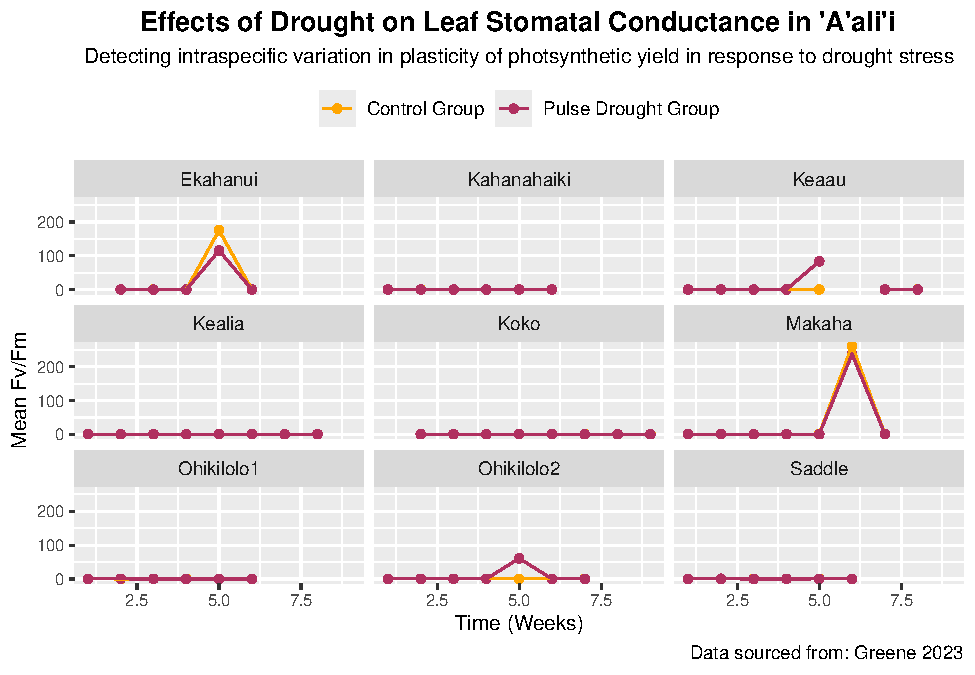
\includegraphics{../Output/unnamed-chunk-3-1.pdf}

\begin{Shaded}
\begin{Highlighting}[]
\NormalTok{npqplot }\OtherTok{\textless{}{-}}\NormalTok{ means }\SpecialCharTok{\%\textgreater{}\%} \CommentTok{\# datasheet}
  \FunctionTok{ggplot}\NormalTok{(}\FunctionTok{aes}\NormalTok{(}\AttributeTok{x =}\NormalTok{ Week, }\CommentTok{\# x{-}axis}
             \AttributeTok{y =}\NormalTok{ mean.npq, }\CommentTok{\# y{-}axis}
             \AttributeTok{color =}\NormalTok{ Treatment)) }\SpecialCharTok{+} \CommentTok{\# colors}
  \FunctionTok{geom\_point}\NormalTok{() }\SpecialCharTok{+}  \CommentTok{\# data points}
  \FunctionTok{geom\_line}\NormalTok{() }\SpecialCharTok{+}  \CommentTok{\# plot}
  \FunctionTok{labs}\NormalTok{(}\AttributeTok{subtitle =} \StringTok{"Detecting intraspecific variation in plasticity of rates of maximum non{-}photochemical quenching values in response to drought stress"}\NormalTok{, }\CommentTok{\# plot subtitle}
       \AttributeTok{caption =} \StringTok{"Data sourced from: Greene 2023"}\NormalTok{, }\CommentTok{\# plot caption}
       \AttributeTok{x =} \StringTok{"Time (Weeks)"}\NormalTok{, }\CommentTok{\# x{-}axis label}
       \AttributeTok{y =} \StringTok{"Mean NPQ Max"}\NormalTok{) }\SpecialCharTok{+} \CommentTok{\# y{-}axis label}
  \FunctionTok{ggtitle}\NormalTok{(}\StringTok{"Effects of Drought on Leaf Stomatal Conductance in \textquotesingle{}A\textquotesingle{}ali\textquotesingle{}i"}\NormalTok{) }\SpecialCharTok{+} \CommentTok{\# plot title}
  \FunctionTok{facet\_wrap}\NormalTok{(}\SpecialCharTok{\textasciitilde{}}\NormalTok{Population) }\SpecialCharTok{+} \CommentTok{\# create panels for each population!}
  \FunctionTok{scale\_color\_manual}\NormalTok{(}\AttributeTok{breaks=} \FunctionTok{c}\NormalTok{(}\StringTok{"C"}\NormalTok{, }\StringTok{"PD"}\NormalTok{), }\AttributeTok{labels =} \FunctionTok{c}\NormalTok{(}\StringTok{"Control Group"}\NormalTok{, }\StringTok{"Pulse Drought Group"}\NormalTok{), }\AttributeTok{values =} \FunctionTok{c}\NormalTok{(}\StringTok{"violet"}\NormalTok{, }\StringTok{"maroon"}\NormalTok{)) }\SpecialCharTok{+} \CommentTok{\# rename legend variables}
  \FunctionTok{theme}\NormalTok{(}\AttributeTok{plot.title =} \FunctionTok{element\_text}\NormalTok{(}\AttributeTok{face =} \StringTok{"bold"}\NormalTok{, }\AttributeTok{color =} \StringTok{"black"}\NormalTok{, }\AttributeTok{hjust =} \FloatTok{0.5}\NormalTok{), }\CommentTok{\# bold title}
        \AttributeTok{axis.text.x =} \FunctionTok{element\_text}\NormalTok{(}\AttributeTok{size =} \DecValTok{8}\NormalTok{), }\AttributeTok{axis.title.x =} \FunctionTok{element\_text}\NormalTok{(}\AttributeTok{size =} \DecValTok{10}\NormalTok{), }\CommentTok{\# adjust x{-}axis labels}
        \AttributeTok{axis.text.y =} \FunctionTok{element\_text}\NormalTok{(}\AttributeTok{size =} \DecValTok{8}\NormalTok{), }\AttributeTok{axis.title.y =} \FunctionTok{element\_text}\NormalTok{(}\AttributeTok{size =} \DecValTok{10}\NormalTok{),   }\CommentTok{\# adjust y{-}axis labels}
        \AttributeTok{legend.position =} \StringTok{"top"}\NormalTok{, }
        \AttributeTok{plot.subtitle =} \FunctionTok{element\_text}\NormalTok{(}\AttributeTok{size =} \DecValTok{10}\NormalTok{, }\AttributeTok{hjust =} \FloatTok{0.5}\NormalTok{), }
        \AttributeTok{legend.title =} \FunctionTok{element\_blank}\NormalTok{())}

\CommentTok{\# save plot to my output folder}
\FunctionTok{ggsave}\NormalTok{(}\FunctionTok{here}\NormalTok{(}\StringTok{"Project"}\NormalTok{, }\StringTok{"Output"}\NormalTok{, }\StringTok{"npqplot.png"}\NormalTok{)) }

\CommentTok{\# view plot}
\NormalTok{npqplot}
\end{Highlighting}
\end{Shaded}

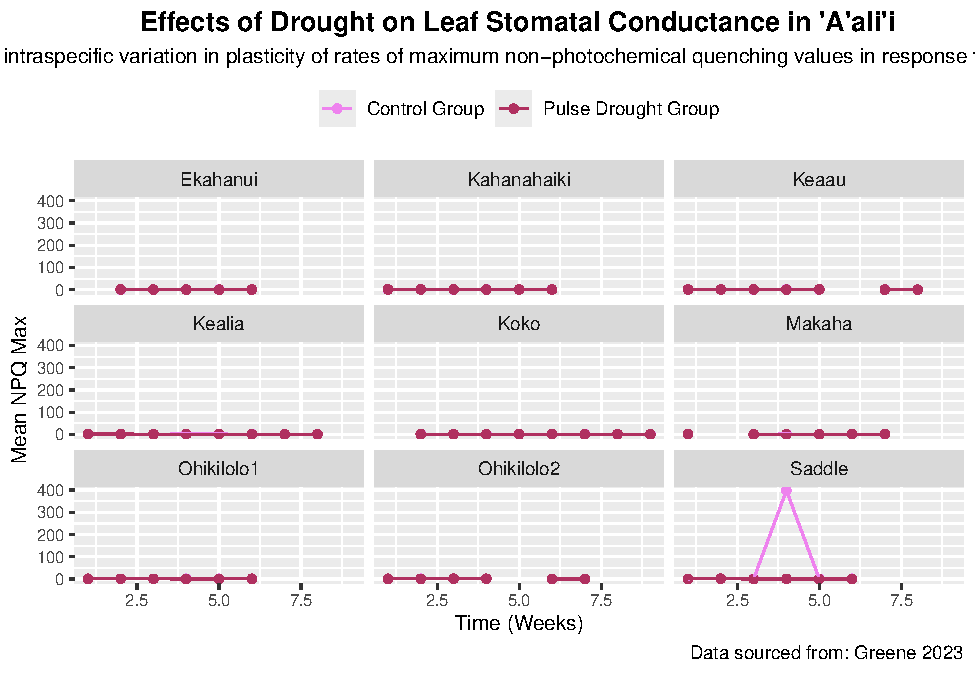
\includegraphics{../Output/unnamed-chunk-4-1.pdf}

\section{Statistic Modeling:
Chlorophyll}\label{statistic-modeling-chlorophyll}

\begin{itemize}
\tightlist
\item
  PT.I: Primary interaction treatment\\
\item
  PT.II: Reduced models\\
\item
  PT.III: Comparison models
\end{itemize}

Data notes:\\
- Effects of Drought Treatment on Chlorophyll Content (F-stat in drought
column)\\
- Code developed with Kasey (with advice from Amber and Kyle):
2024-10-25.\\
- Running the code with the (1\textbar Week:Treatment) interaction and
anova stuff.\\
- Name of model: chl.primary.A/B (untransformed/log-transformed data for
primary interaction) - Chlorophyll: trait of focus\\
- Treatment: fixed factor (drought)\\
- Population: random factor\\
- Population * Treatment: random interaction\\
- Week * Treatment: fixed?? idk. Must ask Kasey.

\begin{Shaded}
\begin{Highlighting}[]
\CommentTok{\# PT.I  }

\CommentTok{\# PRIMARY INTERACTION TREATMENT: UNTRANSFORMED DATA!  }
\CommentTok{\# The F{-}statistic will be the final value for our Drought column in our results table.}
\CommentTok{\# RESULT: F{-}stat: 3.5275}

\NormalTok{chl.primary.A }\OtherTok{=} \FunctionTok{lmer}\NormalTok{(Chlorophyll }\SpecialCharTok{\textasciitilde{}}\NormalTok{ Treatment }\SpecialCharTok{+}\NormalTok{ (}\DecValTok{1}\SpecialCharTok{|}\NormalTok{Week) }\SpecialCharTok{+}\NormalTok{ (}\DecValTok{1}\SpecialCharTok{|}\NormalTok{ID) }\SpecialCharTok{+}\NormalTok{ (}\DecValTok{1}\SpecialCharTok{|}\NormalTok{Population) }\SpecialCharTok{+}\NormalTok{ (}\DecValTok{1}\SpecialCharTok{|}\NormalTok{Population}\SpecialCharTok{:}\NormalTok{Treatment) }\SpecialCharTok{+}\NormalTok{ (}\DecValTok{1}\SpecialCharTok{|}\NormalTok{Population}\SpecialCharTok{:}\NormalTok{Treatment}\SpecialCharTok{:}\NormalTok{Week), }\AttributeTok{data =}\NormalTok{ cleandata)}

\FunctionTok{Anova}\NormalTok{(chl.primary.A, }\AttributeTok{test.statistic =} \StringTok{"F"}\NormalTok{, }\AttributeTok{type =} \DecValTok{3}\NormalTok{)}
\end{Highlighting}
\end{Shaded}

\begin{verbatim}
## Analysis of Deviance Table (Type III Wald F tests with Kenward-Roger df)
## 
## Response: Chlorophyll
##                    F Df  Df.res    Pr(>F)    
## (Intercept) 775.2496  1 10.5566 3.181e-11 ***
## Treatment     3.5275  1  7.6588   0.09882 .  
## ---
## Signif. codes:  0 '***' 0.001 '**' 0.01 '*' 0.05 '.' 0.1 ' ' 1
\end{verbatim}

\begin{Shaded}
\begin{Highlighting}[]
\CommentTok{\# ANOVA RESULTS (POP + TREATMENT INTERACTION)}
\CommentTok{\# Analysis of Deviance Table (Type III Wald F tests with Kenward{-}Roger df)}
\CommentTok{\# Response: Chlorophyll}
                   \CommentTok{\# F Df  Df.res    Pr(\textgreater{}F)    }
\CommentTok{\# (Intercept) 775.2496  1 10.5566 3.181e{-}11 ***}
\CommentTok{\# Treatment     3.5275  1  7.6588   0.09882 .   }
\CommentTok{\# Signif. codes:  0 ‘***’ 0.001 ‘**’ 0.01 ‘*’ 0.05 ‘.’ 0.1 ‘ ’ 1}
\end{Highlighting}
\end{Shaded}

\begin{Shaded}
\begin{Highlighting}[]
\CommentTok{\# NORMALITY CHECK: UNTRANSFORMED  }
  
\CommentTok{\# Shapiro{-}Wilk Normality Test}
\CommentTok{\# Checking normality of residuals in untransformed data}
\CommentTok{\# RESULT: (p{-}value) 1.124e{-}09}

\FunctionTok{shapiro.test}\NormalTok{(}\FunctionTok{resid}\NormalTok{(chl.primary.A)) }
\end{Highlighting}
\end{Shaded}

\begin{verbatim}
## 
##  Shapiro-Wilk normality test
## 
## data:  resid(chl.primary.A)
## W = 0.98397, p-value = 1.124e-09
\end{verbatim}

\begin{Shaded}
\begin{Highlighting}[]
\CommentTok{\# Shapiro{-}Wilk normality test}
\CommentTok{\# data:  resid(chl.primary.A)}
\CommentTok{\# W = 0.98397, p{-}value = 1.124e{-}09}
\end{Highlighting}
\end{Shaded}

\begin{Shaded}
\begin{Highlighting}[]
\CommentTok{\# Untransformed data: QQPlot  }
\FunctionTok{qqnorm}\NormalTok{(}\FunctionTok{resid}\NormalTok{(chl.primary.A))}
\end{Highlighting}
\end{Shaded}

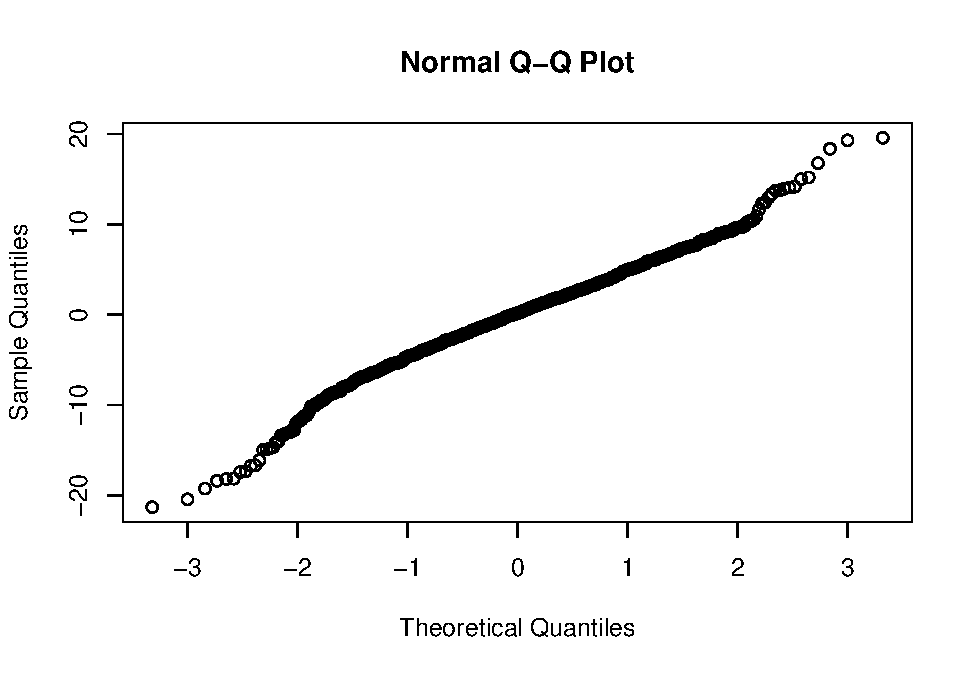
\includegraphics{../Output/unnamed-chunk-6-1.pdf}

\begin{Shaded}
\begin{Highlighting}[]
\CommentTok{\# Log{-}transformed data}
\CommentTok{\# This will be used in the next steps when we look at it as log{-}transformed data.}

\NormalTok{log.chl }\OtherTok{\textless{}{-}} \FunctionTok{log}\NormalTok{(cleandata}\SpecialCharTok{$}\NormalTok{Chlorophyll)}
\FunctionTok{glimpse}\NormalTok{(log.chl)}
\end{Highlighting}
\end{Shaded}

\begin{verbatim}
##  num [1:1107] 3.66 3.28 3.26 3.56 3.53 ...
\end{verbatim}

\begin{Shaded}
\begin{Highlighting}[]
\CommentTok{\# PRIMARY INTERACTION: TRANSFORMED DATA!}
\CommentTok{\# RESULTS: F{-}stat: 0.3662}

\NormalTok{chl.primary.B }\OtherTok{=} \FunctionTok{lmer}\NormalTok{(log.chl }\SpecialCharTok{\textasciitilde{}}\NormalTok{ Treatment }\SpecialCharTok{+}\NormalTok{ (}\DecValTok{1}\SpecialCharTok{|}\NormalTok{Week) }\SpecialCharTok{+}\NormalTok{ (}\DecValTok{1}\SpecialCharTok{|}\NormalTok{ID) }\SpecialCharTok{+}\NormalTok{ (}\DecValTok{1}\SpecialCharTok{|}\NormalTok{Population) }\SpecialCharTok{+}\NormalTok{ (}\DecValTok{1}\SpecialCharTok{|}\NormalTok{Population}\SpecialCharTok{:}\NormalTok{Treatment) }\SpecialCharTok{+}\NormalTok{ (}\DecValTok{1}\SpecialCharTok{|}\NormalTok{Population}\SpecialCharTok{:}\NormalTok{Treatment}\SpecialCharTok{:}\NormalTok{Week), }\AttributeTok{data =}\NormalTok{ cleandata)}

\FunctionTok{Anova}\NormalTok{(chl.primary.B, }\AttributeTok{test.statistic =} \StringTok{"F"}\NormalTok{, }\AttributeTok{type=}\DecValTok{3}\NormalTok{) }
\end{Highlighting}
\end{Shaded}

\begin{verbatim}
## Analysis of Deviance Table (Type III Wald F tests with Kenward-Roger df)
## 
## Response: log.chl
##                     F Df  Df.res    Pr(>F)    
## (Intercept) 5012.0816  1 10.5148 1.976e-15 ***
## Treatment      0.3662  1  7.6474    0.5626    
## ---
## Signif. codes:  0 '***' 0.001 '**' 0.01 '*' 0.05 '.' 0.1 ' ' 1
\end{verbatim}

\begin{Shaded}
\begin{Highlighting}[]
\CommentTok{\# Response: log.chl}
                   \CommentTok{\# F Df  Df.res    Pr(\textgreater{}F)    }
\CommentTok{\# (Intercept) 5012.0816  1 10.5148 1.976e{-}15 ***}
\CommentTok{\# Treatment      0.3662  1  7.6474    0.5626    }
\CommentTok{\# Signif. codes:  0 ‘***’ 0.001 ‘**’ 0.01 ‘*’ 0.05 ‘.’ 0.1 ‘ ’ 1}
\end{Highlighting}
\end{Shaded}

\begin{Shaded}
\begin{Highlighting}[]
\CommentTok{\# NORMALITY CHECK: TRANSFORMED DATA  }

\CommentTok{\# Shapiro{-}Wilk Normality Test  }
\CommentTok{\# Checking normality of residuals in log{-}transformed data}
\CommentTok{\# RESULT: (p{-}value) \textless{} 2.2e{-}16}

\FunctionTok{shapiro.test}\NormalTok{(}\FunctionTok{resid}\NormalTok{(chl.primary.B))}
\end{Highlighting}
\end{Shaded}

\begin{verbatim}
## 
##  Shapiro-Wilk normality test
## 
## data:  resid(chl.primary.B)
## W = 0.8098, p-value < 2.2e-16
\end{verbatim}

\begin{Shaded}
\begin{Highlighting}[]
\CommentTok{\# Shapiro{-}Wilk normality test}
\CommentTok{\# data:  resid(chl.primary.B)}
\CommentTok{\# W = 0.8098, p{-}value \textless{} 2.2e{-}16}
\end{Highlighting}
\end{Shaded}

\begin{Shaded}
\begin{Highlighting}[]
\CommentTok{\# Transformed data: QQPlot }
\FunctionTok{qqnorm}\NormalTok{(}\FunctionTok{resid}\NormalTok{(chl.primary.B))}
\end{Highlighting}
\end{Shaded}

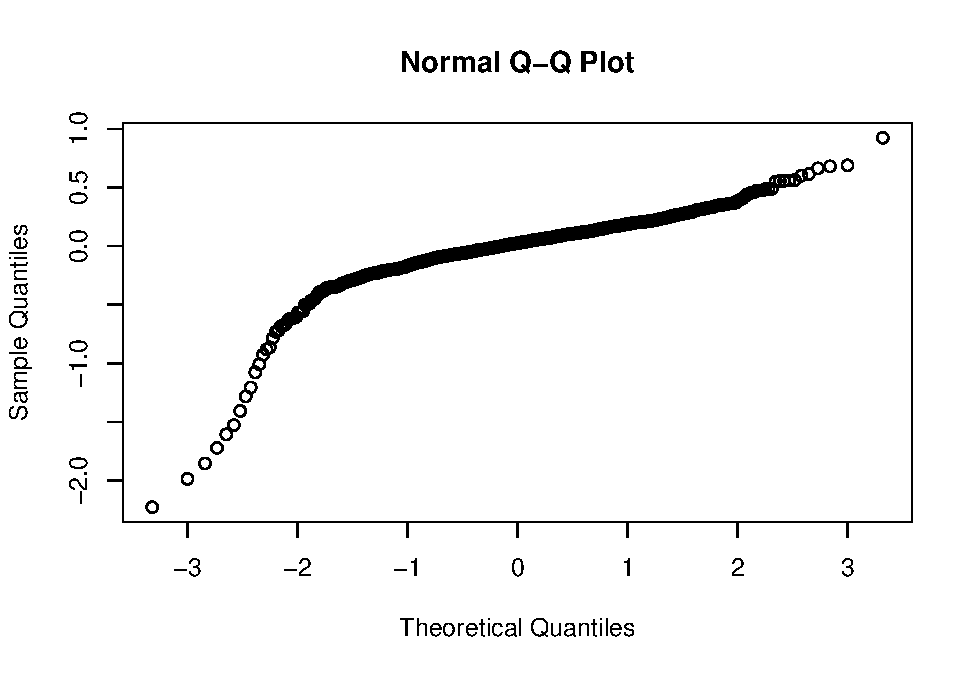
\includegraphics{../Output/unnamed-chunk-10-1.pdf}

\begin{Shaded}
\begin{Highlighting}[]
\CommentTok{\# PT.II   }

\CommentTok{\# REDUCED MODELS!   }
\CommentTok{\# This only tests the effect of Population type on the chlorophyll content results.  }

\NormalTok{chl.reduced.pop }\OtherTok{=} \FunctionTok{lmer}\NormalTok{(Chlorophyll }\SpecialCharTok{\textasciitilde{}}\NormalTok{ Treatment }\SpecialCharTok{+}\NormalTok{ (}\DecValTok{1}\SpecialCharTok{|}\NormalTok{Week) }\SpecialCharTok{+}\NormalTok{ (}\DecValTok{1}\SpecialCharTok{|}\NormalTok{ID) }\SpecialCharTok{+}\NormalTok{ (}\DecValTok{1}\SpecialCharTok{|}\NormalTok{Population), }\AttributeTok{data =}\NormalTok{ cleandata) }
\CommentTok{\# i removed the interaction and treatment in this code so we can just see the population effect}

\FunctionTok{Anova}\NormalTok{(chl.reduced.pop)}
\end{Highlighting}
\end{Shaded}

\begin{verbatim}
## Analysis of Deviance Table (Type II Wald chisquare tests)
## 
## Response: Chlorophyll
##           Chisq Df Pr(>Chisq)  
## Treatment  6.58  1    0.01031 *
## ---
## Signif. codes:  0 '***' 0.001 '**' 0.01 '*' 0.05 '.' 0.1 ' ' 1
\end{verbatim}

\begin{Shaded}
\begin{Highlighting}[]
\CommentTok{\# Analysis of Deviance Table (Type II Wald chisquare tests)}
\CommentTok{\# Response: Chlorophyll}
          \CommentTok{\# Chisq Df Pr(\textgreater{}Chisq)  }
\CommentTok{\# Treatment  6.58  1    0.01031 *}
\CommentTok{\# Signif. codes:  0 ‘***’ 0.001 ‘**’ 0.01 ‘*’ 0.05 ‘.’ 0.1 ‘ ’ 1}
\end{Highlighting}
\end{Shaded}

\begin{Shaded}
\begin{Highlighting}[]
\CommentTok{\# This only tests the effect of pulse drought treatment on the chlorophyll content results}

\NormalTok{chl.reduced.dr }\OtherTok{=} \FunctionTok{glm}\NormalTok{(Chlorophyll }\SpecialCharTok{\textasciitilde{}}\NormalTok{ Treatment, }\AttributeTok{data =}\NormalTok{ cleandata)}
\CommentTok{\# i removed everything but the treatment data so we can see the treatment effect on chlorophyll content results}

\FunctionTok{Anova}\NormalTok{(chl.reduced.dr)}
\end{Highlighting}
\end{Shaded}

\begin{verbatim}
## Analysis of Deviance Table (Type II tests)
## 
## Response: Chlorophyll
##           LR Chisq Df Pr(>Chisq)    
## Treatment   17.769  1  2.494e-05 ***
## ---
## Signif. codes:  0 '***' 0.001 '**' 0.01 '*' 0.05 '.' 0.1 ' ' 1
\end{verbatim}

\begin{Shaded}
\begin{Highlighting}[]
\CommentTok{\# Analysis of Deviance Table (Type II tests)}
\CommentTok{\# Response: Chlorophyll}
          \CommentTok{\# LR Chisq Df Pr(\textgreater{}Chisq)    }
\CommentTok{\# Treatment   17.769  1  2.494e{-}05 ***}
\CommentTok{\# Signif. codes:  0 ‘***’ 0.001 ‘**’ 0.01 ‘*’ 0.05 ‘.’ 0.1 ‘ ’ 1}
\end{Highlighting}
\end{Shaded}

\begin{Shaded}
\begin{Highlighting}[]
\CommentTok{\# PT.III}

\CommentTok{\# COMPARISON MODELS!}
\CommentTok{\# This compares the primary interaction model and population effect reduced model.}
\CommentTok{\# The chisq value will be final result for our P X D column in our table.}
\CommentTok{\# RESULT: 67.711}

\FunctionTok{anova}\NormalTok{(chl.primary.A, chl.reduced.pop)}
\end{Highlighting}
\end{Shaded}

\begin{verbatim}
## Data: cleandata
## Models:
## chl.reduced.pop: Chlorophyll ~ Treatment + (1 | Week) + (1 | ID) + (1 | Population)
## chl.primary.A: Chlorophyll ~ Treatment + (1 | Week) + (1 | ID) + (1 | Population) + (1 | Population:Treatment) + (1 | Population:Treatment:Week)
##                 npar    AIC    BIC  logLik deviance  Chisq Df Pr(>Chisq)    
## chl.reduced.pop    6 7441.4 7471.5 -3714.7   7429.4                         
## chl.primary.A      8 7377.7 7417.8 -3680.9   7361.7 67.711  2  1.981e-15 ***
## ---
## Signif. codes:  0 '***' 0.001 '**' 0.01 '*' 0.05 '.' 0.1 ' ' 1
\end{verbatim}

\begin{Shaded}
\begin{Highlighting}[]
\CommentTok{\# Data: cleandata}
\CommentTok{\# Models:}
\CommentTok{\# chl.reduced.pop: Chlorophyll \textasciitilde{} Treatment + (1 | Week) + (1 | ID) + (1 | Population)}
\CommentTok{\# chl.primary.A: Chlorophyll \textasciitilde{} Treatment + (1 | Week) + (1 | ID) + (1 | Population) + (1 | Population:Treatment) + (1 | Population:Treatment:Week)}

                \CommentTok{\# npar    AIC    BIC  logLik deviance  Chisq Df Pr(\textgreater{}Chisq)    }
\CommentTok{\# chl.reduced.pop    6 7441.4 7471.5 {-}3714.7   7429.4                         }
\CommentTok{\# chl.primary.A      8 7377.7 7417.8 {-}3680.9   7361.7 67.711  2  1.981e{-}15 ***}
\CommentTok{\# Signif. codes:  0 ‘***’ 0.001 ‘**’ 0.01 ‘*’ 0.05 ‘.’ 0.1 ‘ ’ 1}
\end{Highlighting}
\end{Shaded}

\begin{Shaded}
\begin{Highlighting}[]
\CommentTok{\# This compares the population effect reduced model and the treatment effect reduced model.}
\CommentTok{\# The LRT value will be final result for our Population column in our table.}
\CommentTok{\# RESULT: (LRT) }

\CommentTok{\# exactLRT(chl.reduced.pop,chl.reduced.dr) \# LRT (Pop column)}
\end{Highlighting}
\end{Shaded}


\end{document}
